\documentclass[a4paper,12pt]{article}
	\usepackage{fullpage}
	\usepackage[T2A]{fontenc}
	\usepackage[utf8]{inputenc} 
	\usepackage[bulgarian]{babel} 
	\usepackage{graphicx}
	\usepackage{subcaption}
	\usepackage{listings}
	\usepackage{textcomp}
	\usepackage{xcolor}

\title{Бази данни\\Домашна работа}
\author{Ростислав Стоянов  \\ ф-н 45244}
\date{}

\begin{document}
\maketitle 

\textbf {Зад.1} Е/R модел представящ база от данни, съхраняваща информацията искана от условието на задачата, може да се илюстрира чрез E/R диаграмата показана на фиг.1. Приемаме, че един студент може да кандидатства за един изпит само по веднъж, т.е. за всеки изпит, на който кандидат-студентът се явява съществува само по едно заявление. \\

\begin{figure}[h!]
\hspace*{-75pt}
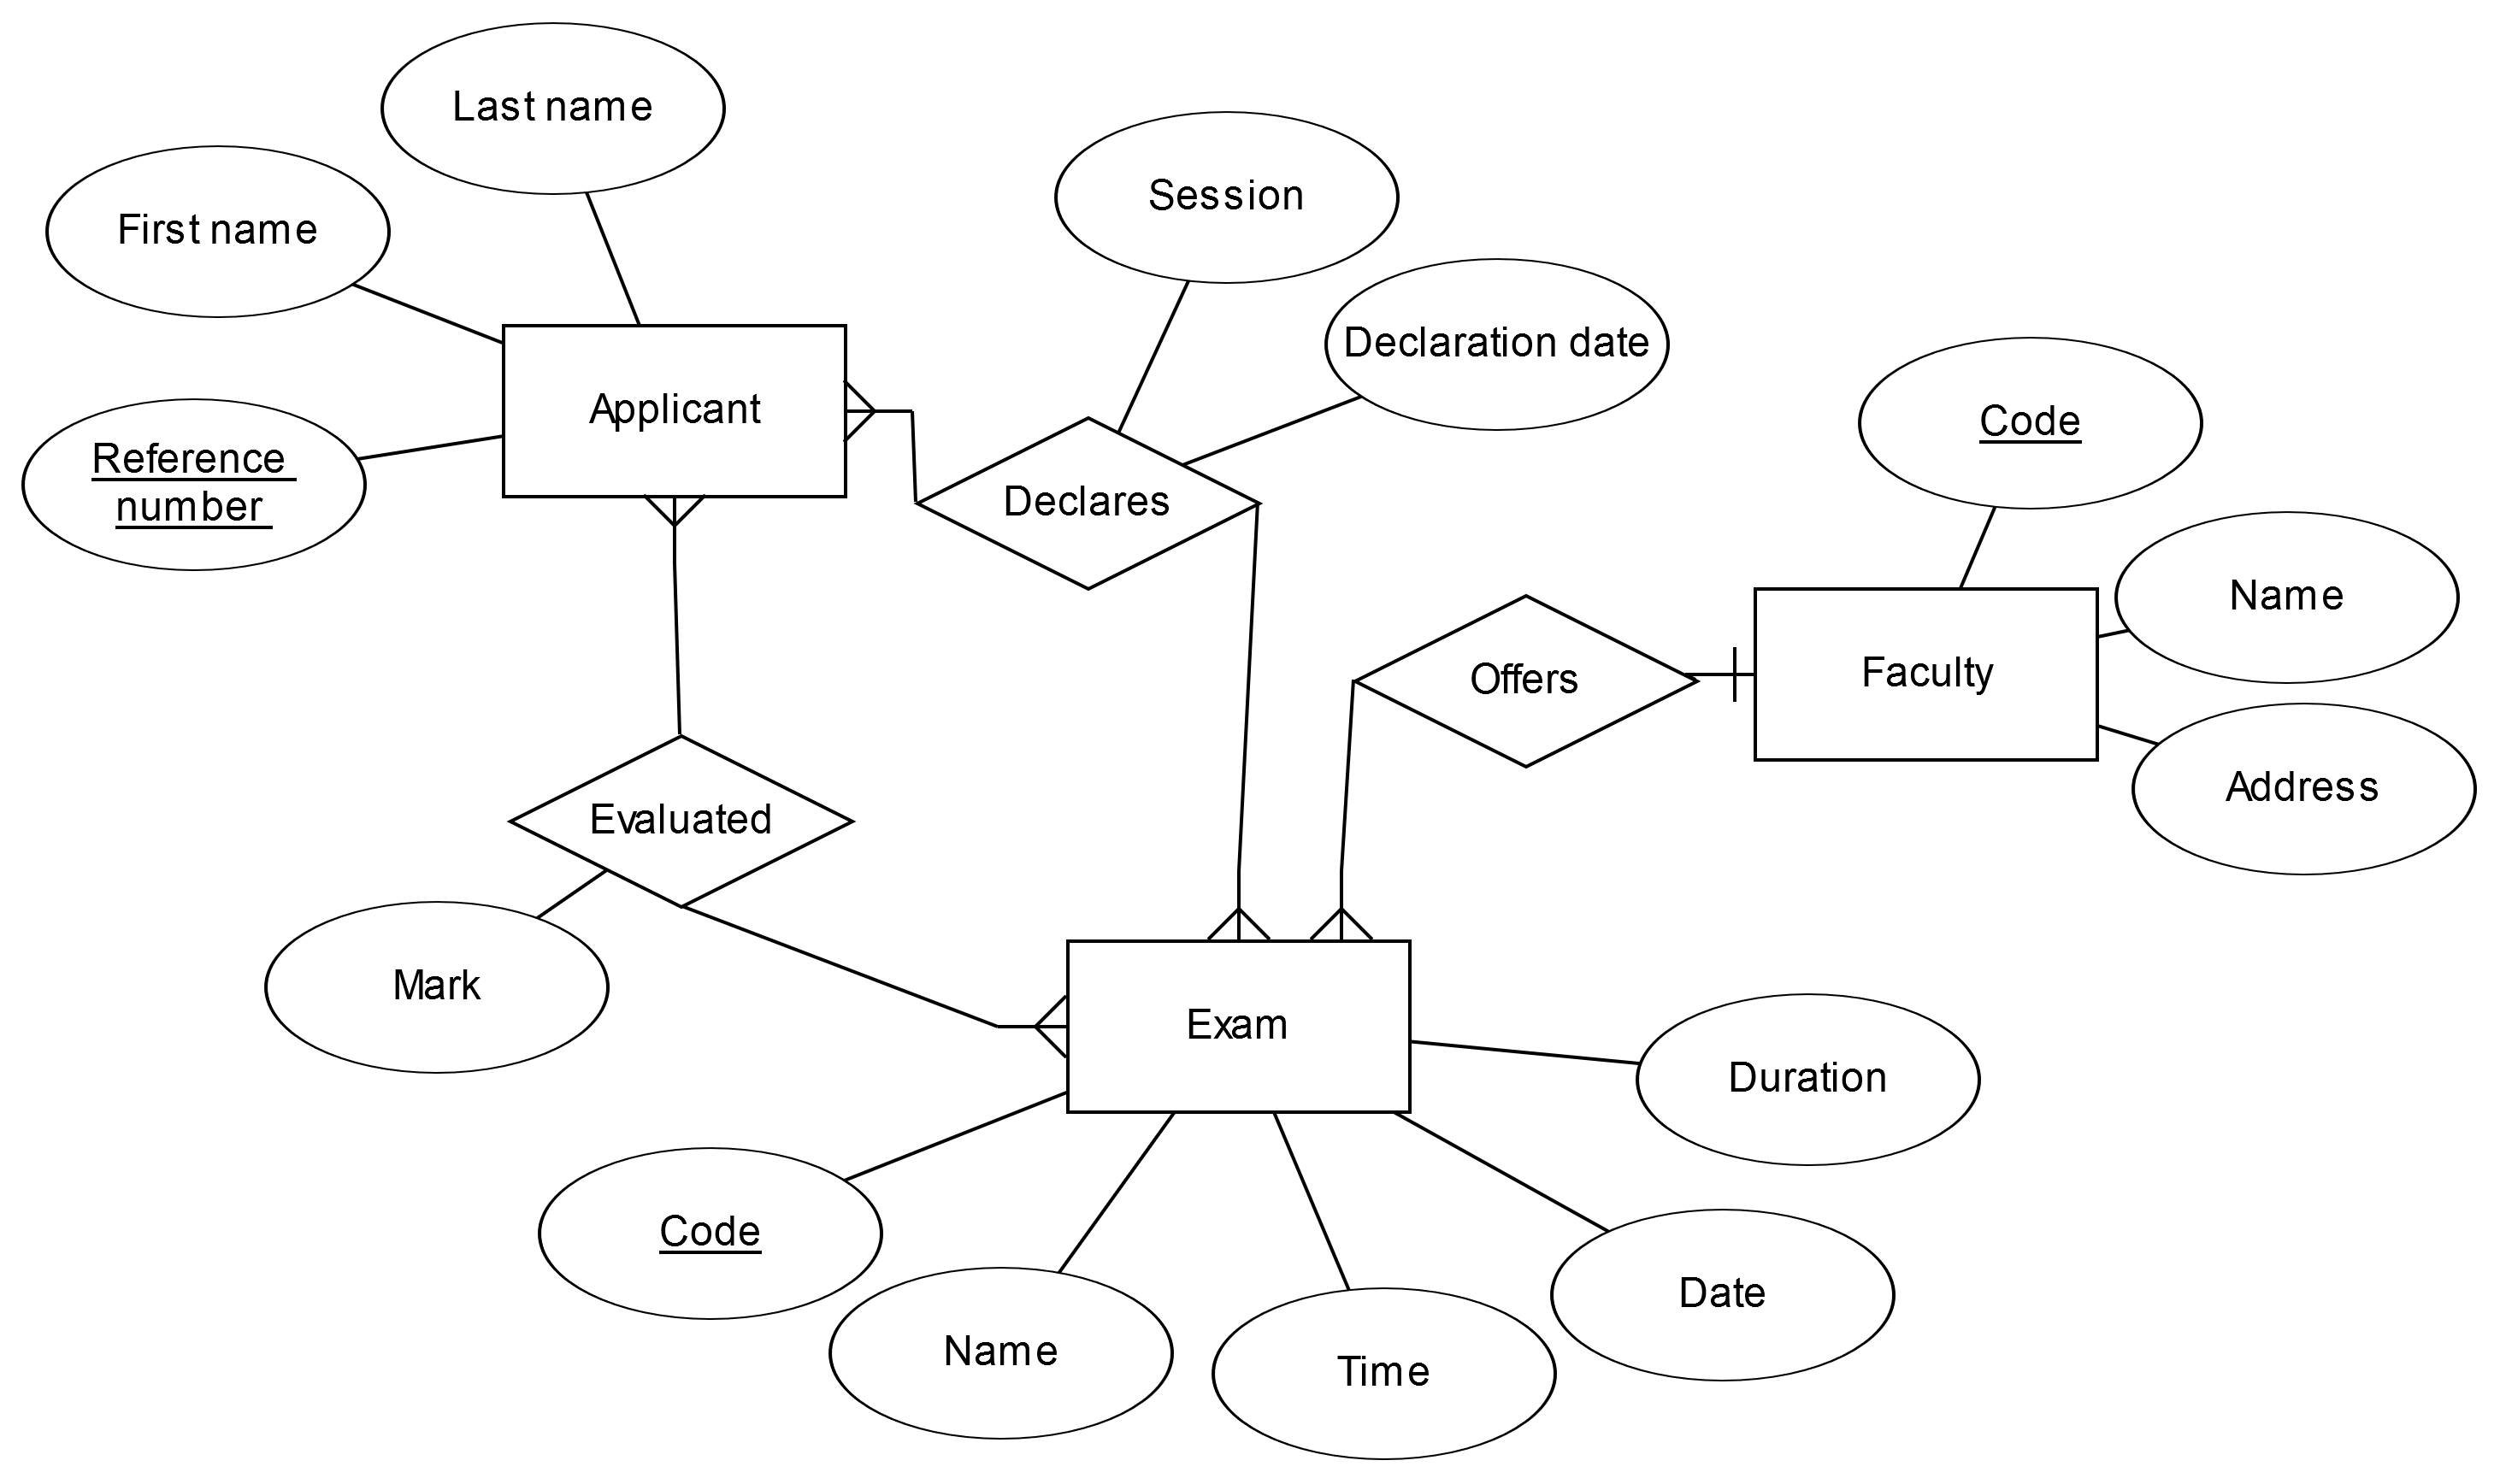
\includegraphics[width=1.32\linewidth]{er.png}
  \caption{E/R диаграма, описваща базата данни от условието}
\end{figure}
\pagebreak

\textbf {Зад.2}
В следствие на преобразуването от E/R към релационен модел, се получават следните релационни схеми:\\
Applicant(\underline{refNumber}, fName, lName), \\
Exam(\underline{examCode},name, time,date duration), \\
Faculty(\underline{facultyCode},name,address),\\
Declares(\underline{applicantNumber}, \underline{examCode}, date, session),\\
Evaluated(\underline{applicantNumber}, \underline{examCode}, mark), \\
Offers(\underline{facultyCode}, \underline{examCode}). \\

Поради факта, че Offers е от вида много-един, след оптимизация получаваме следния релационен модел: \\
Applicant(\underline{refNumber}, fName, lName), \\
Exam(\underline{examCode},name, time,date duration, facultyCode), \\
Faculty(\underline{facultyCode},name,address),\\
Declares(\underline{applicantNumber}, \underline{examCode}, date, session),\\
Evaluated(\underline{applicantNumber}, \underline{examCode}, mark). \\

Първичните ключове са:\\
 \{refNumber\} за Applicant,\\
\{examCode\} за Exam,\\
\{facultyCode\} за Faculty,\\
\{applicantNumber, examCode\} за Declares, \\
\{applicantNumber, examCode\} за Evaluated. \\
\\

Атрибутът applicantNumber в релациите Declares и Evaluated е външен ключ, свързващ ги с релацията Applicant, а атрибутът examCode в същите релации също е външен ключ, свързващ ги с релацията Exam. Външен ключ за Exam е facultyCode, който свързва релацията с Faculty.\\
\begin{figure}[b!]
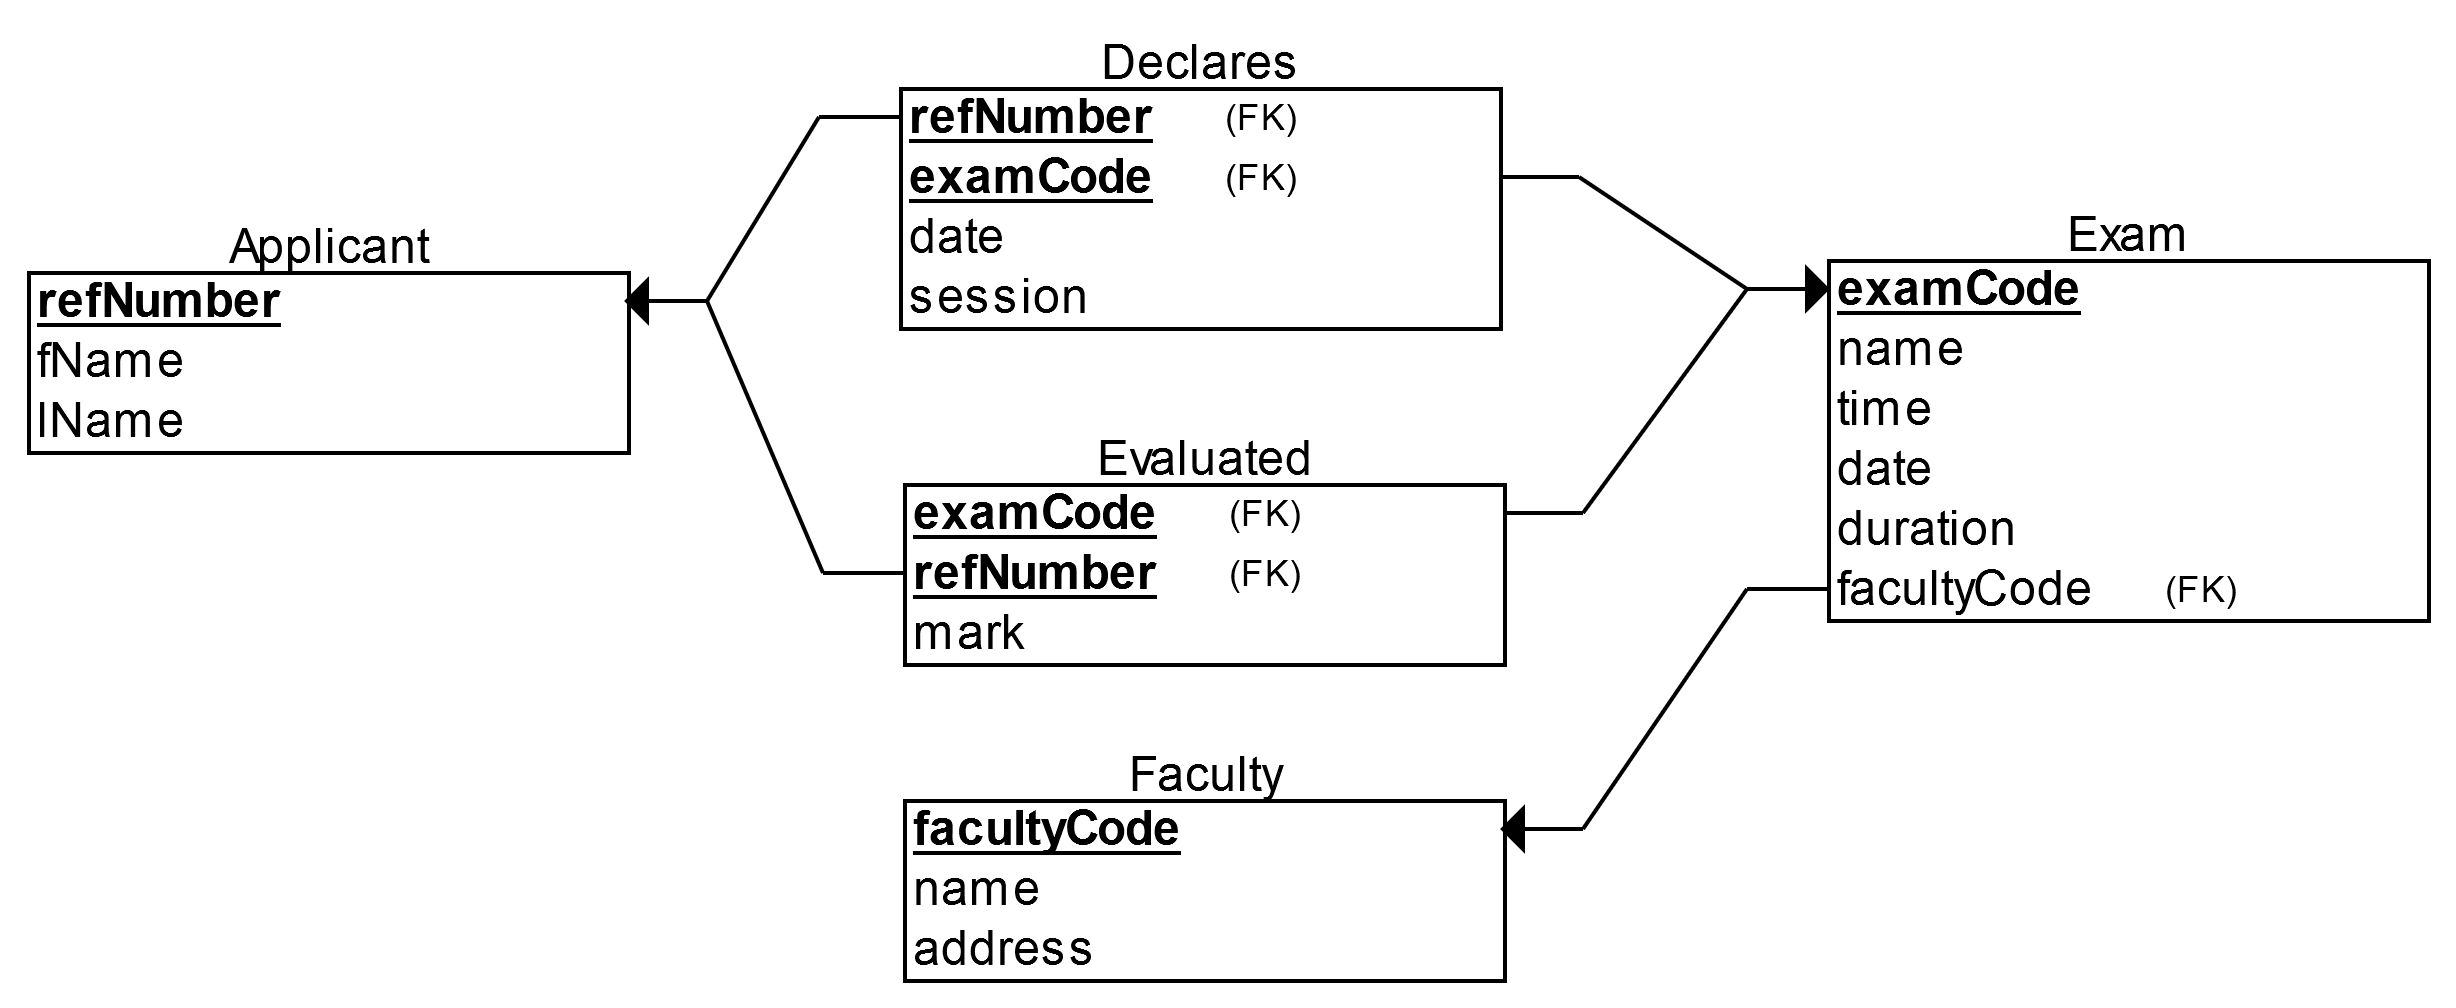
\includegraphics[width=1\linewidth]{rel.png}
  \caption{Релационен модел, описващ базата данни}
\end{figure}
\pagebreak

\textbf {Зад.3}
Фунционални зависимости:
\begin{enumerate}
\item Applicant:
\begin {itemize}
\item\textit{refNumber $\rightarrow$ fName, lName}
\item \textit{refNumber, fName $\rightarrow$ lName}
\item \textit{refNumber, lName $\rightarrow$ fName}
\end{itemize}
Всеки компонент в кортежите на релацията има атомарна стойност $\longrightarrow$ релацията е в 1НФ, но освен това и всеки атрибут е зависим от refNumber,който е единствения атрибут съставляващ първичния ключ $\longrightarrow$ релацията е в 2НФ. Тъй като и лявата част на всяка от функционалните зависимост(първата функционална зависимост може да се раздели на две ФЗ) е суперключ за релацията и тя е в 2НФ, то релацията е в 3НФ.
\item Faculty:
\begin{itemize}
\item\textit{facultyCode $\rightarrow$ name, address}
\item \textit{facultyCode, name $\rightarrow$ address}
\item \textit{facultyCode, address $\rightarrow$ name}
\end{itemize}
Аналогично тук също се извършват проверки (по подобие на извършените при релацията Applicant). Установява се, че и тази релация е в 3НФ.
\item Exam:
\begin{itemize}
\item\textit{examCode $\rightarrow$ name, time, date, duration, facultyCode}
\item \textit{examCode, name $\rightarrow$ name, time, date, duration,facultyCode}
\item \textit{examCode, facultyCode $\rightarrow$ name, time, date, duration}
\item \textit{examCode, facultyCode, name$\rightarrow$time, date, duration}
\item\textit{name, time, date, duration, facultyCode $\rightarrow$ examCode }
\end{itemize}
Атомарната стойност на атрибутите и факта, че ключът на релацията се състои само от examCode, ни водят до 2НФ. За всички ФЗ, без последната, лявата част е суперключ, а за последната ФЗ е изпълнено, че дясната част е част(в частност целия) от ключа, т.е. релацията е в 3НФ.
\item Declares: 
\begin{itemize}
\item \textit{refNumber,examCode $\rightarrow$ date, session}
\item \textit{refNumber,examCode, date $\rightarrow$ session}
\item \textit{refNumber,examCode, session $\rightarrow$ date}
\end{itemize}
Атомарност  $\longrightarrow$ 1НФ; \{refNumber,examCode\} - ключ, всички атрибути зависят от него, но не и от негово подмножество $\longrightarrow$  2НФ. Лесно се проверява, че релацията е и в 3НФ.\\
\item Evaluated: 
\begin{itemize}
\item \textit{refNumber,examCode $\rightarrow$ mark}
\end{itemize}
Очевидно релацията е в 1НФ и тъй като \{refNumber,examCode\} е ключ, а атрибутите поотделно не са ключ за релацията, то тя е във 2НФ. Оттук, тривиално релацията е и в 3НФ. 
\end{enumerate}

\textbf {Зад.4}
\begin{lstlisting}[
           language=SQL,
           showspaces=false,
           basicstyle=\small\ttfamily,
           numbers=left,
           numberstyle=\tiny,
           commentstyle=\color{gray},
	breaklines=true,
        ]
/*Create tables*/

create table Applicant (
refNumber INT NOT NULL,
fName CHAR(30),
lName CHAR(30)
);

create table Faculty (
facultyCode INT NOT NULL,
name CHAR(50),
address VARCHAR(255)
);

create table Exam(
examCode INT NOT NULL,
name CHAR(50),
time TIME,
date DATE,
duration INT,
facultyCode INT
);

create table Declares(
refNumber INT NOT NULL,
examCode INT NOT NULL,
date DATE,
session CHAR(30) 
);

create table Evaluated(
refNumber INT NOT NULL,
examCode INT NOT NULL,
mark ENUM(2,3,4,5,6)
);

/*Create constraints*/
alter table Applicant add constraint PK_Applicant PRIMARY KEY(refNumber);
alter table Faculty add constraint PK_Faculty PRIMARY KEY(facultyCode);
alter table Exam add constraint PK_Exam PRIMARY KEY(examCode);
alter table Declares add constraint PK_Declares PRIMARY KEY(refNumber,examCode);
alter table Evaluated add constraint PK_Evaluated PRIMARY KEY(refNumber,examCode);

alter table Exam add constraint FK_Exam_Faculty FOREIGN KEY(facultyCode) references Faculty(facultyCode);
alter table Declares add constraint  FK_Declares_Applicant FOREIGN KEY(refNumber) references Applicant(refNumber);
alter table Declares add constraint  FK_Declares_Exam FOREIGN KEY (examCode) references Exam (examCode);
alter table Evaluated add constraint  FK_Evaluated_Applicant FOREIGN KEY(refNumber) references Applicant(refNumber);
alter table Evaluated add constraint   FK_Evaluated_Exam FOREIGN KEY (examCode) references Exam (examCode);
\end{lstlisting}

\end{document}